\begin{figure}[ht!]
\centering
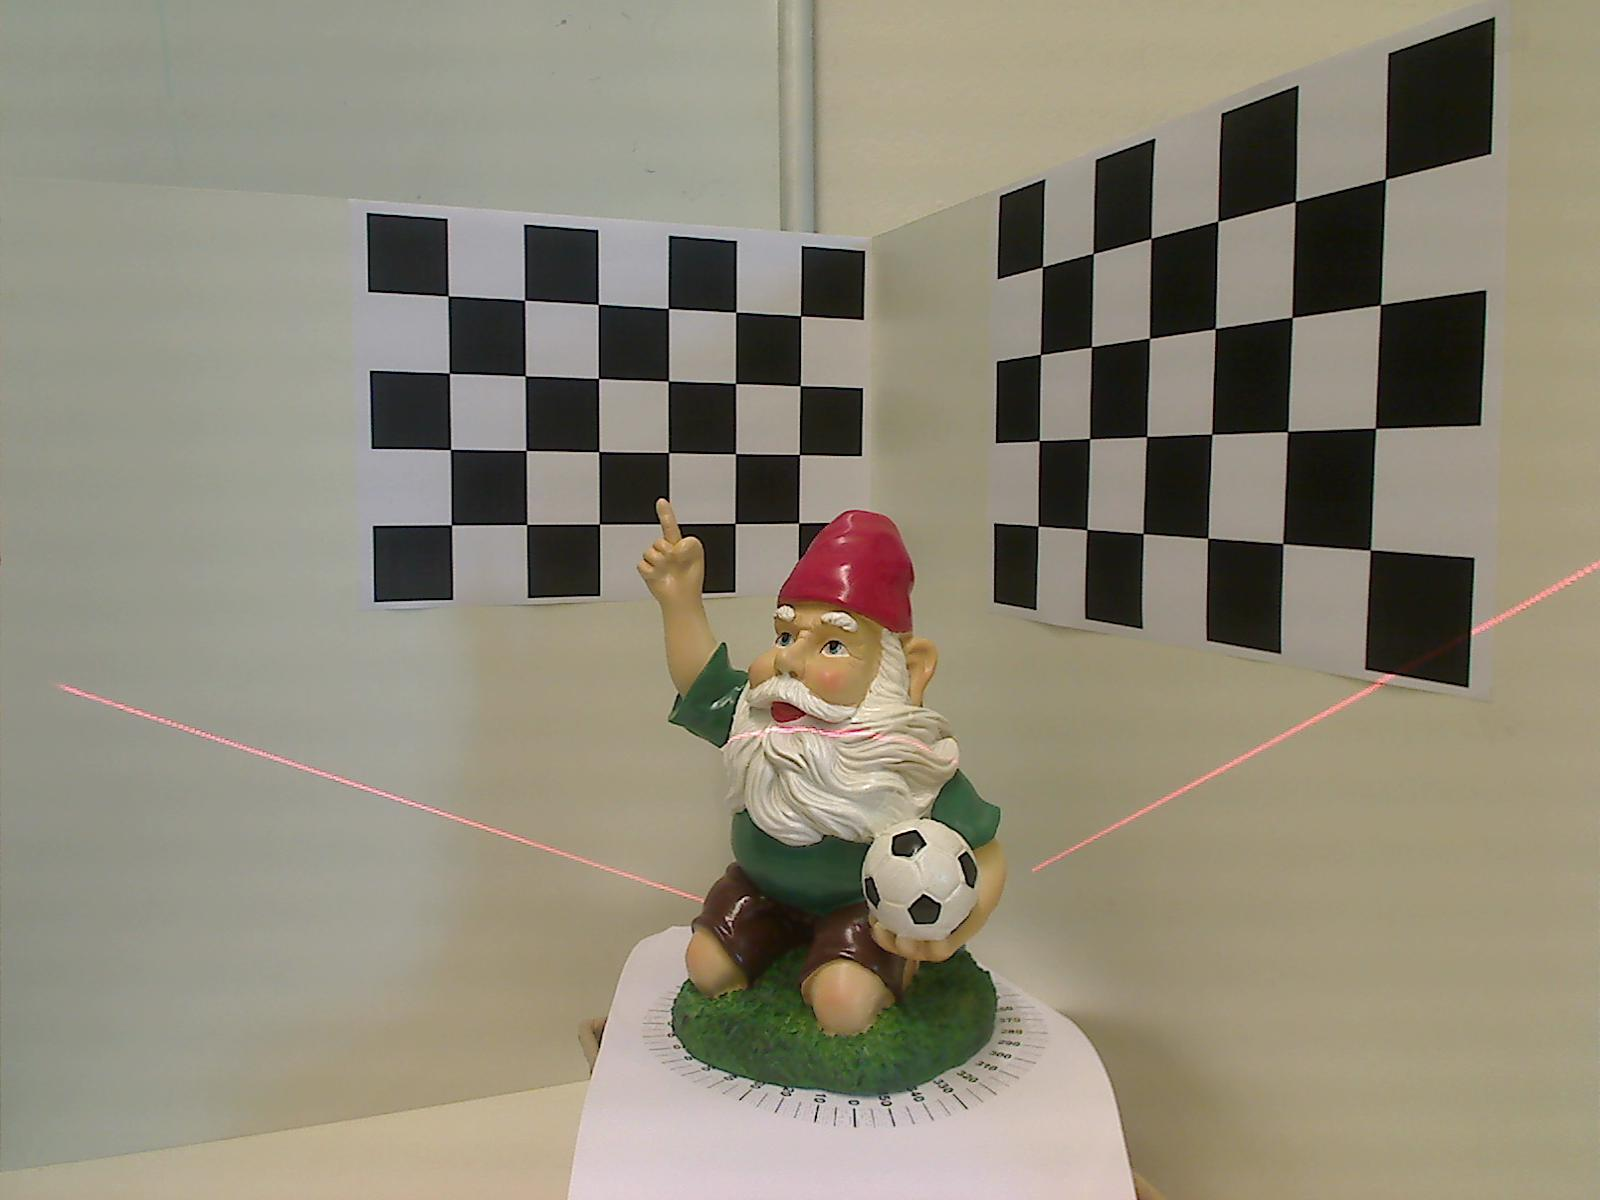
\includegraphics[width=0.5\linewidth]{figures/introduction}
\label{figure:acquisition}
\caption{Data Acquisition}
\end{figure}

We used a standard digital camera to capture multiple runs of a hand-held laser sweeping across the object as shown in figure \ref{figure:acquisition}. Since the videos were stored in raw format which cannot be directly processed by OpenCV, we used \texttt{mplayer} to extract individual frames at the rate of 5 frames per second.

\begin{verbatim}
$ mplayer -demuxer rawvideo \
          -rawvideo fps=5:w=1600:h=1200:yuy2 \
          -vo pnm:ppm $FILE	
\end{verbatim}

These frames were then later read into memory by calling the OpenCV routine \texttt{cvLoadImage()} with a \texttt{CV\_LOAD\_IMAGE\_UNCHANGED} flag. The routine allocates an image data structure and returns a pointer to a struct of type \texttt{IplImage}

